\documentclass[CT4S-EN-RU]{subfiles}

\begin{document}

\section{\caseENGRUS{Operads}{ / }{Операды}}\label{sec:operad}

\begin{blockENG}
In this section we briefly introduce operads, which are generalizations of categories. They often are useful for speaking about self-similarity of structure. For example, we will use them to model agents made up of smaller agents, or materials made up of smaller materials. This association with self-similarity is not really inherent in the definition, but it tends to emerge in our thinking about many operads used in practice. 
\end{blockENG}

\begin{blockRUS}
\end{blockRUS}

\begin{blockENG}
Let me begin with a warning.
\end{blockENG}

\begin{blockRUS}
\end{blockRUS}

\begin{warningENG}\index{a warning!operads vs. multicategories}
My use of the term operad is not entirely standard and conflicts with widespread usage. The more common term for what I am calling an operad is {\em symmetric colored operad} or a {\em symmetric multicategory}\index{multicategory}\index{operad!colored}. An operad classically is a multicategory with one object, and a colored operad is a multicategory. The analogy is that “operad is to multicategory as monoid is to category”. The term multicategory stems from the fact that the morphisms in a multicategory have many, rather than one, input. But there is nothing really “multi” about the multicategory itself, only its morphisms. Probably the real reason though is that I find the term multicategory to be clunky and the term operad to be sleek, clocking in at half the syllables. I apologize if my break with standard terminology causes any confusion.  
\end{warningENG}

\begin{warningRUS}\index{a warning!operads vs. multicategories}
\end{warningRUS}

\begin{blockENG}
This introduction to operads is quite short. One should see \cite{Le1} for an excellent treatment.
\end{blockENG}

\begin{blockRUS}
\end{blockRUS}

%%%% Subsection %%%%

\subsection{\caseENGRUS{Definition and classical examples}{ / }{Определение и классические примеры}}

\begin{blockENG}
An operad is like a category in that it has objects, morphisms, and a composition formula, and it follows an identity law and an associativity law. The difference is that each morphism has many inputs (and one output).
\begin{center}
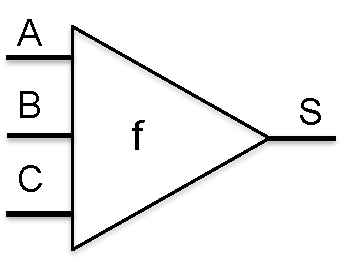
\includegraphics[height=1in]{operadArrow}
\end{center}
The description of composition in an operad is a bit heavier than it is in a category, but the idea fairly straightforward. Here is a picture of morphisms being composed.
\begin{center}
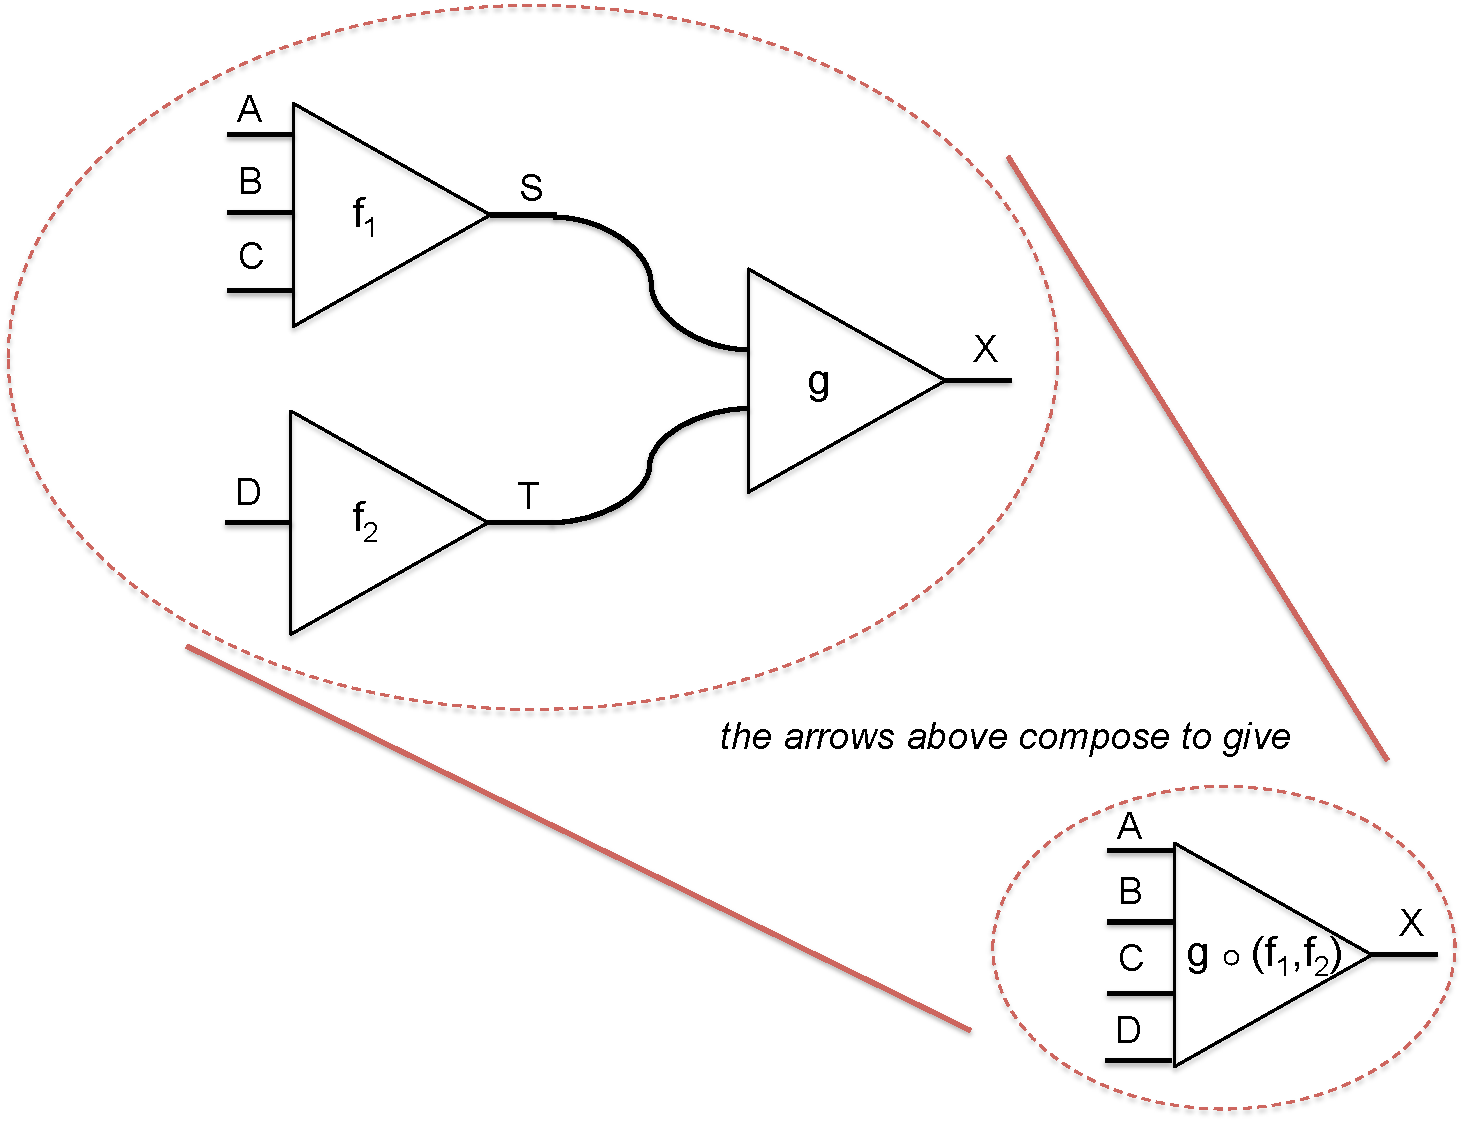
\includegraphics[width=\textwidth]{operadComposition}
\end{center}
Note that $S$ and $T$ disappear from the composition, but this is analogous to the way the middle object disappears from the composition of morphisms in a category
$$\color{Maroon}\dashbox{\color{black}$A\Too{f}S\Too{g} X$} \color{black}\hsp\tn{\em the arrows to the left compose to give}\hsp \color{Maroon}\dashbox{\color{black}$A\Too{g\circ f}X$}$$
Here is the definition, which we take directly from \cite{Sp4}.
\end{blockENG}

\begin{blockRUS}
\end{blockRUS}

\begin{definitionENG}\label{def:operad}
An {\em operad} $\mcO$ is defined as follows: One announces some constituents (A. objects, B. morphisms, C. identities, D. compositions) and asserts that they conform to some laws (1. identity law, 2. associativity law). Specifically, 
\begin{enumerate}[\hsp A.]
\item one announces a collection $\Ob(\mcO),$ each element of which is called an {\em object} of $\mcO.$
\item for each object $y\in\Ob(\mcO),$ finite set $n\in\Ob(\Fin),$ and $n$-indexed set of objects $x\taking n\to\Ob(\mcO),$ one announces a set $\mcO_n(x;y)\in\Ob(\Set).$ Its elements are called {\em morphisms from $x$ to $y$} in $\mcO.$ 
\item for every object $x\in\Ob(\mcO),$ one announces a specified morphism denoted $\id_x\in\mcO_1(x;x)$ called {\em the identity morphism on $x$}.
\item Let $s\taking m\to n$ be a morphism in $\Fin.$ Let $z\in\Ob(\mcO)$ be an object, let $y\taking n\to\Ob(\mcO)$ be an $n$-indexed set of objects, and let $x\taking m\to\Ob(\mcO)$ be an $m$-indexed set of objects. For each element $i\in n,$ write $m_i:=s^\m1(i)$ for the pre-image of $s$ under $i,$ and write $x_i=x|_{m_i}\taking m_i\to\Ob(\mcO)$ for the restriction of $x$ to $m_i.$ Then one announces a function 
\begin{align}\label{dia:composition formula}
\circ\taking\mcO_n(y;z)\times\prod_{i\in n}\mcO_{m_i}(x_i;y(i))\too\mcO_{m}(x;z),
\end{align} 
called {\em the composition formula}.
\end{enumerate}
Given an $n$-indexed set of objects $x\taking n\to\Ob(\mcO)$ and an object $y\in\Ob(\mcO),$ we sometimes abuse notation and denote the set of morphisms from $x$ to $y$ by $\mcO(x_1,\ldots,x_n;y).$
\footnote{There are three abuses of notation when writing $\mcO(x_1,\ldots,x_n;y),$ which we will fix one by one. First, it confuses the set $n\in\Ob(\Fin)$ with its cardinality $|n|\in\NN.$ But rather than writing $\mcO(x_1,\ldots,x_{|n|};y),$ it would be more consistent to write $\mcO(x(1),\ldots,x(|n|);y),$ because we have assigned subscripts another meaning in part D. But even this notation unfoundedly suggests that the set $n$ has been endowed with a linear ordering, which it has not. This may be seen as a more serious abuse, but see Remark~\ref{rem:symmetry}.}
We may write $\Hom_\mcO(x_1,\ldots,x_n;y),$ in place of $\mcO(x_1,\ldots,x_n;y),$ when convenient. We can denote a morphism $\phi\in\mcO_n(x;y)$ by $\phi\taking x\to y$ or by $\phi\taking (x_1,\ldots,x_n)\to y$; we say that each $x_i$ is a {\em domain object} of $\phi$ and that $y$ is the {\em codomain object} of $\phi.$ We use infix notation for the composition formula, e.g. writing $\psi\circ(\phi_1,\ldots,\phi_n).$

One asserts that the following laws hold:
\begin{enumerate}[\hsp 1.]
\item for every $x_1,\ldots,x_n,y\in\Ob(\mcO)$ and every morphism $\phi\taking(x_1,\ldots,x_n)\to y,$ we have
$$\phi\circ(\id_{x_1},\ldots,\id_{x_n})=\phi\hsp\tn{and}\hsp\id_y\circ\phi=\phi;$$
\item Let $m\To{s}n\To{t}p$ be composable morphisms in $\Fin.$ Let $z\in\Ob(\mcO)$ be an object, let $y\taking p\to\Ob(\mcO),$ $x\taking n\to\Ob(\mcO),$ and $w\taking m\to\Ob(\mcO)$ respectively be a $p$-indexed, $n$-indexed, and $m$-indexed set of objects. For each $i\in p,$ write $n_i=t^\m1(i)$ for the pre-image and $x_i\taking n_i\to\Ob(\mcO)$ for the restriction. Similarly, for each $k\in n$ write $m_k=s^\m1(k)$ and $w_k\taking m_k\to\Ob(\mcO)$; for each $i\in p,$ write $m_{i,-}=(t\circ s)^\m1(i)$ and $w_{i,-}\taking m_{i,-}\to\Ob(\mcO)$; for each $j\in n_i,$ write $m_{i,j}:=s^\m1(j)$ and $w_{i,j}\taking m_{i,j}\to\Ob(\mcO).$ Then the diagram below commutes:
$$\hspace{-1.4in}\xymatrix@=18pt{
&
{\hspace{.9in}\color{white}\prod\color{black}}
\save[]+<0cm,0cm>*\txt<30pc>{$
\mcO_p(y;z)\times\prod_{i\in p}\mcO_{n_i}(x_i;y(i))\times\prod_{i\in p,\ j\in n_i}\mcO_{m_{i,j}}(w_{i,j};x_i(j))
$}
\ar[rd]\ar[ld]
\restore\\
{\hspace{1in}\color{white}\prod\color{black}}
\save[]+<.4cm,0cm>*\txt<30pc>{$
\mcO_n(x;z)\times\prod_{k\in n}\mcO_{m_k}(w_k;x(k))
$}
\ar[dr]
\restore&&
{\hspace{1in}\color{white}\prod\color{black}}
\save[]+<-.3cm,0cm>*\txt<30pc>{$
\mcO_p(y;z)\times\prod_{i\in p}\mcO_{m_{i,-}}(w_{i,-};y(i))
$}
\ar[dl]
\restore\\
&\mcO_m(w;z)
}
$$
\end{enumerate}
\end{definitionENG}

\begin{definitionRUS}\label{def:operad}
\end{definitionRUS}

\begin{remarkENG}\label{rem:symmetry}
In this remark we will discuss the abuse of notation in Definition~\ref{def:operad} and how it relates to an action of a symmetric group on each morphism set in our definition of operad. We follow the notation of Definition~\ref{def:operad}, especially following the use of subscripts in the composition formula.

Suppose that $\mcO$ is an operad, $z\in\Ob(\mcO)$ is an object, $y\taking n\to\Ob(\mcO)$ is an $n$-indexed set of objects, and $\phi\taking y\to z$ is a morphism. If we linearly order $n,$ enabling us to write $\phi\taking (y(1),\ldots,y(|n|))\to z,$ then changing the linear ordering amounts to finding an isomorphism of finite sets $\sigma\taking m\To{\iso} n,$ where $|m|=|n|.$ Let $x=y\circ\sigma$ and for each $i\in n,$ note that $m_i=\sigma^\m1(\{i\})=\{\sigma^\m1(i)\},$ so $x_i=x|_{\sigma^\m1(i)}=y(i).$ Taking $\id_{x_i}\in\mcO_{m_i}(x_i;y(i))$ for each $i\in n,$ and using the identity law, we find that the composition formula induces a bijection $\mcO_n(y;z)\To{\iso}\mcO_m(x;z),$ which we might denote by 
$$\sigma\taking\mcO(y(1),y(2),\ldots,y(n);z)\iso\mcO\big(y(\sigma(1)),y(\sigma(2)),\ldots,y(\sigma(n));z\big).$$
In other words, there is an induced group action of $\Aut(n)$ on $\mcO_n(x;z),$ where $\Aut(n)$ is the group of permutations of an $n$-element set.

Throughout this book, we will permit ourselves to abuse notation and speak of morphisms $\phi\taking (x_1,x_2,\ldots,x_n)\to y$ for a natural number $n\in\NN,$ without mentioning the abuse inherent in choosing an order, so long as it is clear that permuting the order of indices would not change anything up to canonical isomorphism.
\end{remarkENG}

\begin{remarkRUS}\label{rem:symmetry}
\end{remarkRUS}

\begin{exampleENG}\index{an operad!$\Sets$}
Let $\Sets$ denote the operad defined as follows. For objects we put $\Ob(\Sets)=\Ob(\Set).$ For a natural number $n\in\NN$ and sets $X_1,\ldots,X_n,Y,$ put 
$$\Hom_\Sets(X_1,\ldots,X_n;Y):=\Hom_\Set(X_1\times\cdots\times X_n,Y).$$
Given functions $f_1\taking(X_{1,1}\times\cdots\times X_{1,m_1})\to Y_1$ through $f_n\taking (X_{n,1}\times\cdots\times X_{n,m_n})\to Y_n$ and a function $Y_1\times\cdots\times Y_n\to Z,$ the universal property provides us a unique function of the form $(X_{1,1}\times\cdots\times X_{n,m_n})\too Z,$ giving rise to our composition formula.
\end{exampleENG}

\begin{exampleRUS}\index{an operad!$\Sets$}
\end{exampleRUS}

\begin{exampleENG}[Little squares operad]\label{ex:little squares}\index{an operad!little squares}
An operad commonly used in mathematics is called the {\em little $n$-cubes operad}\index{an operad!little $n$-cubes}. We'll focus on $n=2$ and talk about the little squares operad $\mcO.$ Here the set of objects has only one element, which we denote by a square, $\Ob(\mcO)=\{\square\}.$ For a natural number $n\in\NN,$ a morphism $f\taking(\square,\square,\ldots,\square)\too\square$ is a positioning of $n$ non-overlapping squares inside of a square. Here is a picture of a morphism $(X_1,X_2,X_3)\to Y,$ where $X_1=X_2=X_3=Y=\square.$
\begin{center}
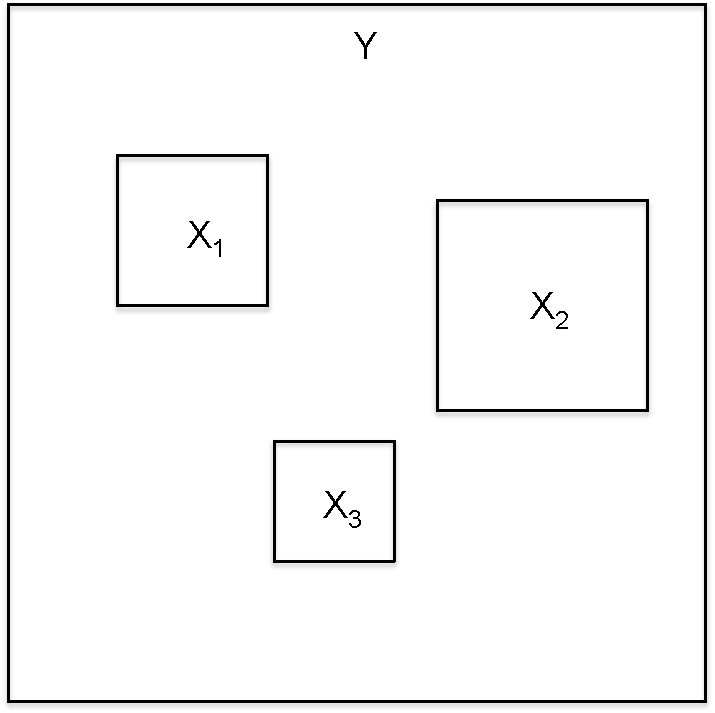
\includegraphics[height=2in]{square1}
\end{center}
The composition law says that given a positioning of small squares inside a large square, and given a positioning of tiny squares inside each of those small squares, we get a positioning of tiny squares inside a large square. A picture is shown in Figure~\ref{fig:composition law for squares}.
\begin{figure}[H]
\begin{center}
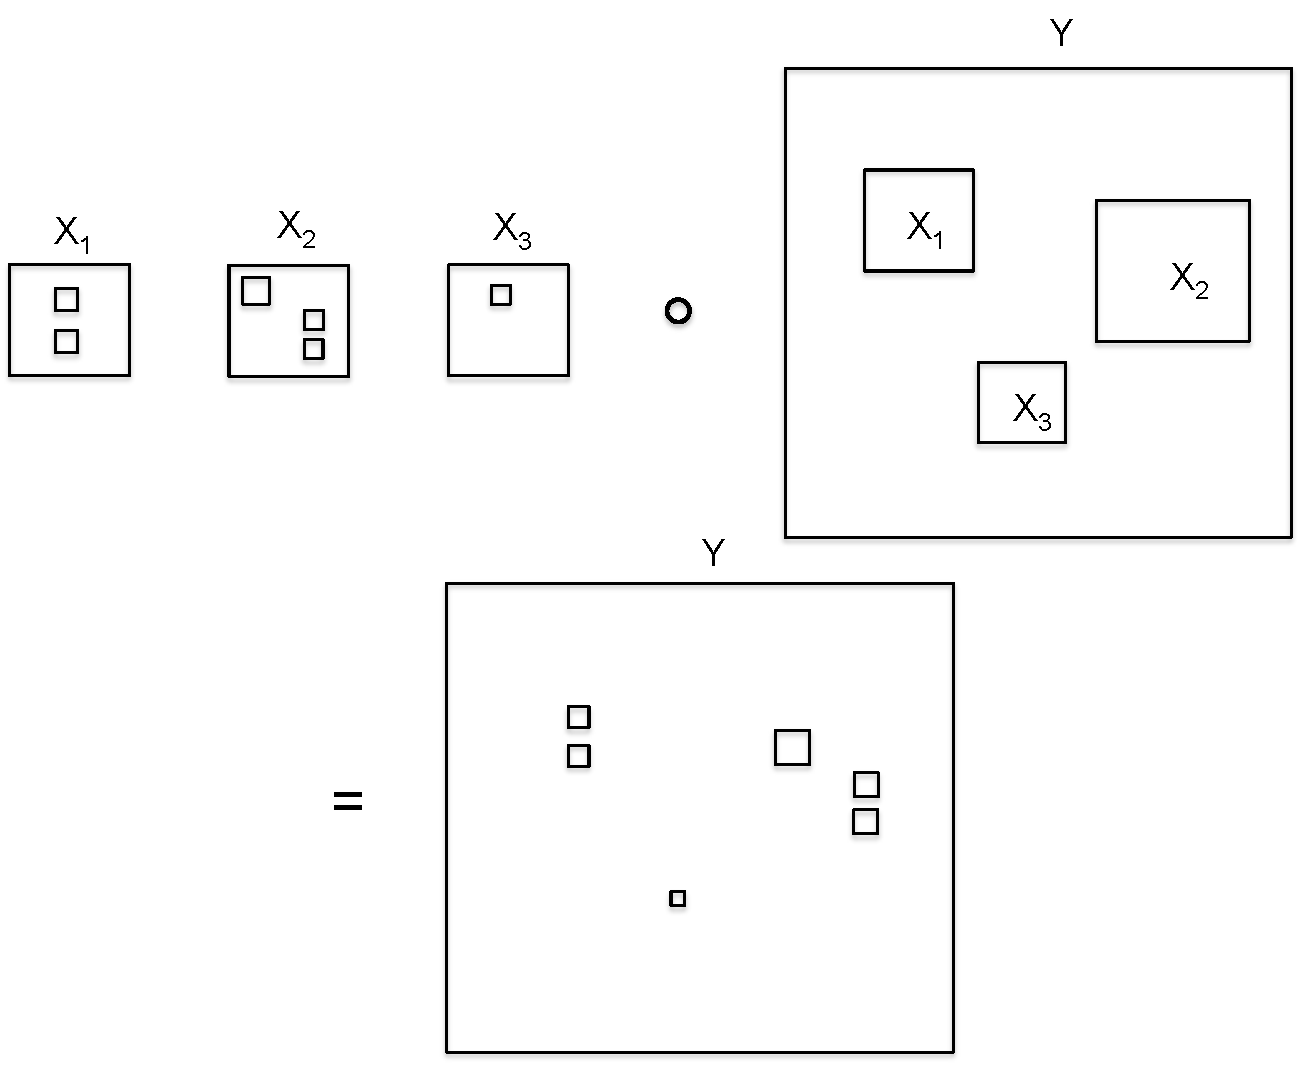
\includegraphics[width=\textwidth]{square2}
\end{center}
\caption{Here we show a morphism $(X_1,X_2,X_3)\to Y$ and morphisms $(W_{1,1},W_{1,2})\to X_1,$ $(W_{2,1},W_{2,2},W_{2,3})\to X_2,$ and $(W_{3,1})\to X_3,$ each of which is a positioning of squares inside a square. The composition law scales and positions the squares in the “obvious” way.}
\label{fig:composition law for squares}
\end{figure}

Hopefully, what we meant by “self-similarity” in the introduction to this section (see page \pageref{sec:operad}) is becoming clear.
\end{exampleENG}

\begin{exampleRUS}[Little squares operad]\label{ex:little squares}\index{an operad!little squares}
\end{exampleRUS}

\begin{exerciseENG}\label{exc:little shapes}
Consider an operad $\mcO$ like the little squares operad from Example~\ref{ex:little squares}, except with three objects: square, circle, equilateral triangle. A morphism is again a non-overlapping positioning of shapes inside of a shape. 
\sexc Draw an example of a morphism $f$ from two circles and a square to a triangle.
\item Find three other morphisms that compose into $f,$ and draw the composite.
\endsexc
\end{exerciseENG}

\begin{exerciseRUS}\label{exc:little shapes}
\end{exerciseRUS}

%% Subsubsection %%

\subsubsection{\caseENGRUS{Operads: functors and algebras}{ / }{Операды: функторы и алгебры}}

\begin{blockENG}
If operads are like categories, then we can define things like functors and call them {\em operad functors}. Before giving the definition, we give a warning.
\end{blockENG}

\begin{blockRUS}
\end{blockRUS}

\begin{warningENG}\index{a warning!operad functors}
What we call operad functors in Definition~\ref{def:operad morphism} are usually (if not always) called {\em operad morphisms}. We thought that the terminology clash between morphisms {\em of} operads and morphisms {\em in} an operad was too confusing. It is similar to what would occur in regular category theory (e.g. Chapter~\ref{chap:categories}) if we replaced the term “functor” with the term “category morphism”. 
\end{warningENG}

\begin{warningRUS}\index{a warning!operad functors}
\end{warningRUS}

\begin{definitionENG}\label{def:operad morphism}\index{operad!morphism of}
Let $\mcO$ and $\mcO'$ be operads. An {\em operad functor from $\mcO$ to $\mcO'$}, denoted $F\taking\mcO\to\mcO'$ consists of some constituents (A. on-objects part, B. on-morphisms part) conforming to some laws (1. preservation of identities, 2. preservation of composition), as follows:
\begin{enumerate}[\hsp A.]
\item There is a function $\Ob(F)\taking\Ob(\mcO)\to\Ob(\mcO').$
\item For each object $y\in\Ob(\mcO),$ finite set $n\in\Ob(\Fin),$ and $n$-indexed set of objects $x\taking n\to\Ob(\mcO),$ there is a function $$F_n\taking\mcO_n(x;y)\to\mcO'_n(Fx;Fy).$$
\end{enumerate}
As in B. above, we often denote $\Ob(F),$ and also each $F_n,$ simply by $F.$ The laws that govern these constituents are as follows:
\begin{enumerate}[\hsp 1.]
\item For each object $x\in\Ob(\mcO),$ the equation $F(\id_x)=\id_{Fx}$ holds.
\item Let $s\taking m\to n$ be a morphism in $\Fin.$ Let $z\in\Ob(\mcO)$ be an object, let $y\taking n\to\Ob(\mcO)$ be an $n$-indexed set of objects, and let $x\taking m\to\Ob(\mcO)$ be an $m$-indexed set of objects. Then, with notation as in Definition~\ref{def:operad}, the following diagram of sets commutes:
\begin{align}\label{dia:operad functor on composition}
\xymatrix{
\mcO_n(y;z)\times\prod_{i\in n}\mcO_{m_i}(x_i;y(i))\ar[r]^-F\ar[d]_\circ&
\mcO'_n(Fy;Fz)\times\prod_{i\in n}\mcO'_{m_i}(Fx_i;Fy(i))\ar[d]^\circ\\
\mcO_m(x;z)\ar[r]_F&\mcO'_m(Fx;Fz)
}
\end{align}
\end{enumerate}

We denote the category of operads and operad functors by $\Oprd.$
\end{definitionENG}

\begin{definitionRUS}\label{def:operad morphism}\index{operad!morphism of}
\end{definitionRUS}

\begin{exerciseENG}
Let $\mcO$ denote the little squares operad from Example~\ref{ex:little squares} and let $\mcO'$ denote the operad you constructed in Exercise~\ref{exc:little shapes}.
\sexc Can you come up with an operad functor $\mcO\to\mcO'?$
\item Is it possible to find an operad functor $\mcO'\to\mcO?$ 
\endsexc
\end{exerciseENG}

\begin{exerciseRUS}
\end{exerciseRUS}

\begin{definitionENG}[Operad algebra]\label{def:operad algebra}\index{algebra!operad}\index{operad!algebra of}
Let $\mcO$ be an operad. An {\em algebra on $\mcO$} is an operad functor $A\taking\mcO\to\Sets.$
\end{definitionENG}

\begin{definitionRUS}[Operad algebra]\label{def:operad algebra}\index{algebra!operad}\index{operad!algebra of}
\end{definitionRUS}

\begin{remarkENG}
Every category can be construed as an operad (yes, there is a functor $\Cat\to\Oprd$), by simply not including non-unary morphisms. That is, given a category $\mcC,$ one makes an operad $\mcO$ with $\Ob(\mcO):=\Ob(\mcC)$ and with 
$$
\Hom_\mcO(x_1,\ldots,x_n;y)=
\begin{cases}
\Hom_\mcC(x_1,y)&\tn{ if }n=1;\\
\emptyset&\tn{ if }n\neq 1
\end{cases}
$$
Just like a schema is a category presentation, it is possible to discuss operad presentations by generators and relations. Under this analogy, an algebra on an operad corresponds to an instance on a schema.
\end{remarkENG}

\begin{remarkRUS}
\end{remarkRUS}

%%%% Subsection %%%%

\subsection{\caseENGRUS{Applications of operads and their algebras}{ / }{Применения операд и их алгебр}}

\begin{blockENG}
Hierarchical structures may be well-modeled by operads. Describing such structures using operads and their algebras allows one to make appropriate distinctions between different types of thinking. For example, the allowable formations are encoded in the operad, whereas the elements that will fit into those formations are encoded in the algebra. Morphisms of algebras are high-level understandings of how elements of very different types (such as materials vs. numbers) can occupy the same place in the structure and be compared. We will give examples below.
\end{blockENG}

\begin{blockRUS}
\end{blockRUS}

\begin{applicationENG}
\href{http://en.wikipedia.org/wiki/Composite_material}{\text Every material is composed of constituent materials}, arranged in certain patterns. (In case the material is “pure”, we consider the material to consist of itself as the sole constituent.) Each of these constituent materials each is itself an arrangement of constituent materials. Thus we see a kind of self-similarity which we can model with operads. 

\begin{align}\label{dia:material comp}
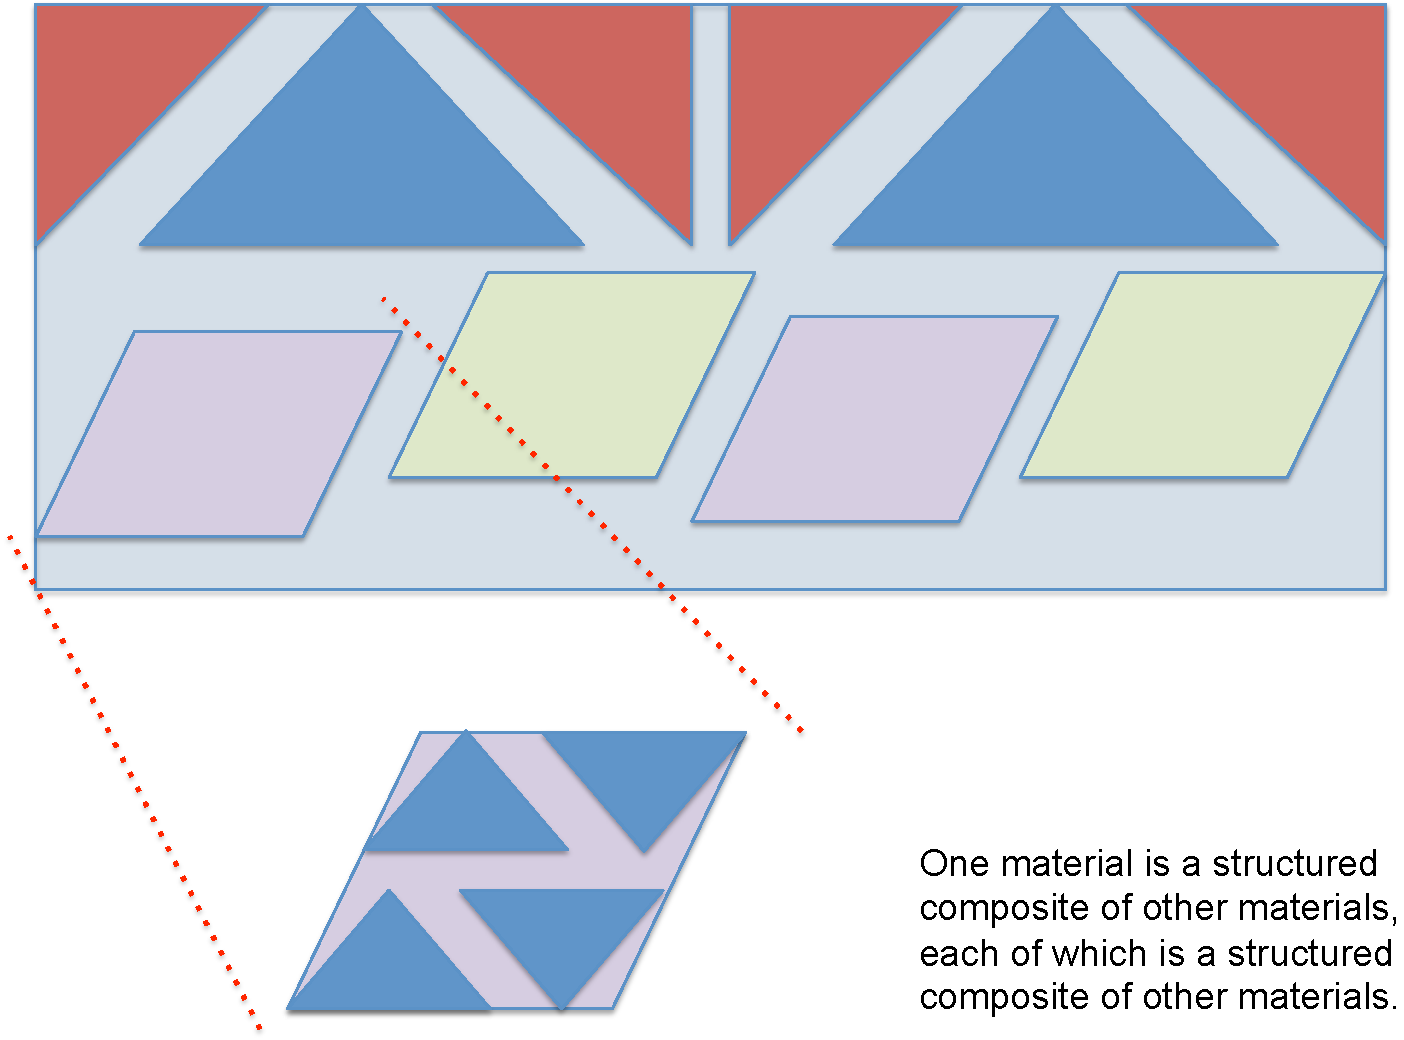
\includegraphics[width=\textwidth]{materialComposition}
\end{align}

For example, a tendon is made of collagen fibers that are assembled in series and then in parallel, in a specific way. Each collagen fibre is made of collagen fibrils that are again assembled in series and then in parallel, with slightly different specifications. We can continue down, perhaps indefinitely, though our resolution fails at some point. A collagen fibril is made up of tropocollagen collagen molecules, which are twisted ropes of collagen molecules, etc.\footnote{Thanks to Professor Sandra Shefelbine for explaining the hierarchical nature of collagen to me. Any errors are my own.}

Here is how operads might be employed. We want the same operad to model both actual materials, theoretical materials, and functional properties; that is we want more than one algebra on the same operad. 

The operad $\mcO$ should abstractly model the structure, but not the substance being structured. Imagine that each of the shapes (including the background “shape”) in Diagram (\ref{dia:material comp}) is a place-holder, saying something like “{\em your material here}”. Each morphism (that's what (\ref{dia:material comp}) is a picture of) represents a construction of a material out of parts. In our picture, it appears we are only concerned with the spacial arrangements, but there is far more flexibility than that. Whether we want to allow for additional details beyond spacial arrangements is the kinds of choice we make in a meeting called “what operad should we use?” 
\end{applicationENG}

\begin{applicationRUS}
\end{applicationRUS}

\begin{applicationENG}
Suppose we have chosen an operad $\mcO$ to model the structure of materials. Each object of $\mcO$ might correspond to a certain quality of material, and each morphism corresponds to an arrangement of various qualities to form a new quality. An algebra $A\taking\mcO\to\Sets$ on $\mcO$ forces us to choose what substances will fill in for these qualities. For every object $x\in\Ob(\mcO),$ we want a set $A(x)$ which will be the set of materials with that quality. For every arrangement, i.e. morphism, $f\taking (x_1,\ldots,x_n)\to y,$ and every choice $a_1\in A(x_1), \ldots, a_n\in A(x_n)$ of materials, we need to understand what material $a'=A(f)(a_1,\ldots,a_n)\in A(y)$ will emerge when these materials are arranged in accordance with $f.$ We are really pinning ourselves down here.

But there may be more than one interesting algebra on $\mcO.$ Suppose that $B\taking\mcO\to\Sets$ is an algebra of strengths rather than materials. For each object $x\in\Ob(\mcO),$ which represents some quality, we let $B(x)$ be the set of possible strengths that something of quality $x$ can have. Then for each arrangement, i.e. morphism, $f\taking (x_1,\ldots,x_n)\to y,$ and every choice $b_1\in B(x_1), \ldots, b_n\in B(x_n)$ of strengths, we need to understand what strength $b'=B(f)(b_1,\ldots,b_n)\in B(y)$ will emerge when these strengths are arranged in accordance with $f.$ Certainly an impressive achievement!

Finally, a morphism of algebras $S\taking A\to B$ would consist of a coherent system for assigning to each material $a\in A(X)$ of a given quality $x$ a specific strength $S(a)\in B(X),$ in such a way that morphisms behaved appropriately. In this language we have stated a very precise goal for the field of material mechanics.
\end{applicationENG}

\begin{applicationRUS}
\end{applicationRUS}

\begin{exerciseENG}
Consider again the little squares operad $\mcO$ from Example~\ref{ex:little squares}. Suppose we wanted to use this operad to describe those \href{http://en.wikipedia.org/wiki/Photographic_mosaic}{\text photographic mosaics}. 
\sexc Come up with an algebra $P\taking\mcO\to\Sets$ that sends the square to the set of all photos that can be pasted into that square. What does $P$ do on morphisms in $\mcO?$
\item Come up with an algebra $C\taking\mcO\to\Sets$ that sends each square to the set of all colors (visible frequencies of light). In other words, $C(\square)$ is the set of colors, not the set of ways to color the square. What does $C$ do on morphisms in $\mcO.$ Hint: use some kind of averaging scheme for the morphisms.
\item Guess: if someone were to appropriately define morphisms of $\mcO$-algebras (something akin to natural transformations between functors $\mcO\to\Sets$), do you think there would some a morphism of algebras $P\to C?$
\endsexc
\end{exerciseENG}

\begin{exerciseRUS}
\end{exerciseRUS}

%% Subsubsection %%

\subsubsection{\caseENGRUS{Wiring diagrams}{ / }{Проволочные диаграммы}}

\begin{exampleENG}\label{ex:operad of relations}
Here we describe an {\em operad of relations}, which we will denote by $\mcR.$ The objects are sets, $\Ob(\mcR)=\Ob(\Set).$ A morphism $f\taking (x_1,x_2,\ldots,x_n)\too x'$ in $\mcR$ is a diagram in $\Set$ of the form 
\begin{align}\label{dia:operad of relations}
\xymatrix@=15pt{&&&R\ar[llldd]_(.7){f_1}\ar[lldd]^{f_2}\ar@{}[ldd]^(.6)\cdots\ar[dd]^(.6){f_n}\ar[rrdd]^(.7){f'}\\\\x_1&x_2&\cdots&x_n&&x'}
\end{align} 
such that the induced function $R\too(x_1\times x_2\times\cdots\times x_n\times x')$ is an injection.

We use a composition formula similar to that in Definition~\ref{def:composite span}. Namely, we form a fiber product
$$\xymatrix{&&FP\ar[rd]\ar[ld]\\&\prod_{i\in\ul{n}}R_i\ar[ld]\ar[rd]&&S\ar[ld]\ar[rd]\\\prod_{i\in\ul{n}}\prod_{j\in\ul{m_i}}x_{i,j}&&\prod_{i\in\ul{n}}y_i&&z}$$
One can show that the induces function $FP\too\left(\prod_{i\in\ul{n}}\prod_{j\in\ul{m_i}}x_i\right)\times y$ is an injection, so we have a valid composition formula. Finally, the associativity and identity laws hold.
\footnote{Technically we need to use isomorphism classes of cone points, but we don't worry about this here.}
\end{exampleENG}

\begin{exampleRUS}\label{ex:operad of relations}
\end{exampleRUS}

\begin{applicationENG}\label{app:entity by experience}
Suppose we are trying to model \href{http://en.wikipedia.org/wiki/Life}{\text life} in the following way. We define an entity as a set of phenomena, but in order to use colloquial language we say the entity {\em is able to experience} that set of phenomena. We also want to be able to put entities together to form a super-entity, so we have a notion of morphism $f\taking(e_1,\ldots,e_n)\too e'$ defined as a relation as in (\ref{dia:operad of relations}). The idea is that the morphism $f$ is a way of translating between the phenomena that may be experienced by the sub-entities and the phenomena that may be experienced by the super-entity. 

The operad $\mcR$ from Example~\ref{ex:operad of relations} becomes useful as a language for discussing issues in this domain.
\end{applicationENG}

\begin{applicationRUS}\label{app:entity by experience}
\end{applicationRUS}

\begin{exampleENG}\label{ex:algebra on operad of rels}
Let $\mcR$ be the operad of relations from Example~\ref{ex:operad of relations}. Consider the algebra $S\taking\mcR\to\Sets$ given by $S(x)=\PP(x).$ Given a morphism $\prod_ix_i\from R\to y$ and subsets $x_i'\ss x_i,$ we have a subset $\prod_ix_i'\ss\prod_ix_i.$ We take the fiber product
$$\xymatrix@=15pt{&FP\ar[rr]\ar[ld]&&R\ar[ld]\ar[rd]\\\prod_ix_i'\ar[rr]&&\prod_ix_i&&y}$$
and the image of $FP\to y$ is a subset of $y.$ 
\end{exampleENG}

\begin{exampleRUS}\label{ex:algebra on operad of rels}
\end{exampleRUS}

\begin{applicationENG}\label{app:desire}
Following Application~\ref{app:entity by experience} we can use Example~\ref{ex:algebra on operad of rels} as a model of survival. Each entity survives only for a subset of the phenomena that it can experience. Under this interpretation, the algebra from Example~\ref{ex:algebra on operad of rels} defines survival as the survival of all parts. That is, suppose that we understand how a super-entity is composed of sub-entities in the sense that we have a translation between the set of phenomena that may be experienced across the sub-entities and the set of phenomena that may be experienced by the super-entity. Then the super-entity will survive exactly those phenomena which translate to phenomena for which each sub-entity desires. 

Perhaps a better term than survival would be “allowance”. A bureaucracy consists of a set of smaller bureaucracies, each of which allows certain phenomena to pass; the whole bureaucracy allows something to pass if and only if, when translated to the perspective of each sub-bureaucracy, it is allowed to pass there.
\end{applicationENG}

\begin{applicationRUS}\label{app:desire}
\end{applicationRUS}

\begin{exampleENG}
In this example we discuss wiring diagrams that look like this:\index{wiring diagram}
\begin{center}
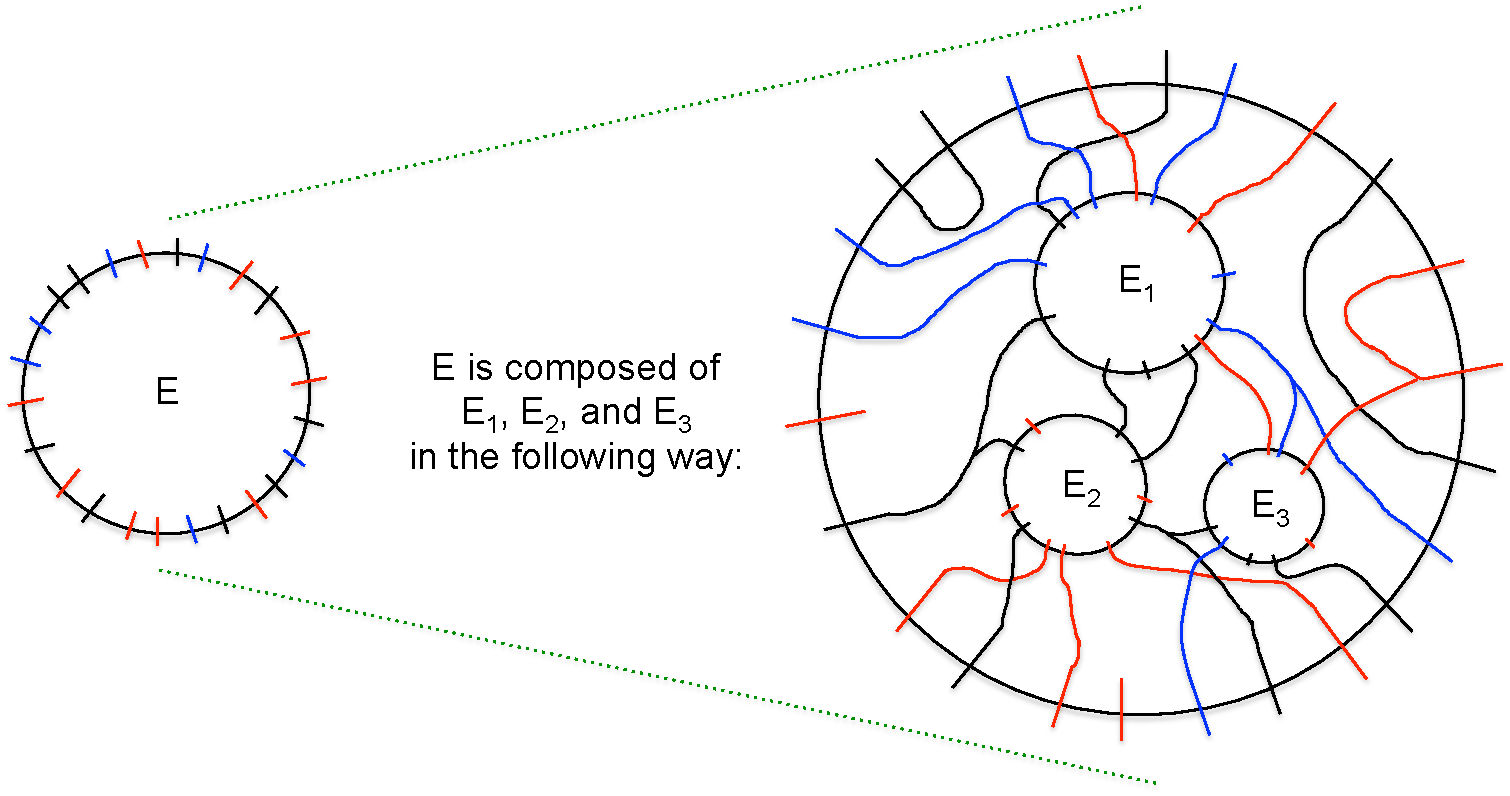
\includegraphics[width=\textwidth]{wiringDiagram}
\end{center}
The operad in question will be denoted $\mcW$; it is discussed in greater detail in \cite{Sp4}. The objects of $\mcW$ are pairs $(C,s)$ where $C$ is a finite set and $v\taking C\to\Ob(\Set)$ is a function. Think of such an object as a circle with $C$-many cables sticking out of it; each cable $c$ is assigned a set $v(c)$ corresponding to the set of values that can be carried on that cable. For example $E_2=(C,v)$ where $|C|=11$ and we consider $v$ to be specified by declaring that black wires carry $\ZZ$ and red wires carry $\{\tn{sweet, sour, salty, bitter, umami}\}.$ 

The morphisms in $\mcW$ will be pictures as above, formalized as follows. Given objects $(C_1,v_1),\ldots,(C_n,v_n), (D,w),$ a morphism $F\taking((C_1,v_1),\ldots,(C_n,v_n))\too (D,w)$ is a commutative diagram of sets
\footnote{If one is concerned with cardinality issues, fix a cardinality $\kappa$ and replace $\Ob(\Set)$ everywhere with $\Ob(\Set_{<\kappa}).$} 
$$
\xymatrix{\bigsqcup_{i\in\ul{n}}C_i\ar[rd]_{\sqcup_iv_i}\ar[r]^i&G\ar[d]^x&D\ar[l]_j\ar[ld]^w\\&\Ob(\Set)}
$$
such that $i$ and $j$ are jointly surjective.

Composition of morphisms is easily understood in pictures: given wiring diagrams inside of wiring diagrams, we can throw away the intermediary circles. In terms of sets, we perform a pushout.

There is an operad functor $\mcW\to\mcS$ given by sending $(C,v)$ to $\prod_{c\in C}v(c).$ The idea is that to an entity defined as having a bunch of cables carrying variables, a phenomenon is the same thing as a choice of value on each cable. A wiring diagram translates between values experienced locally and values experienced globally. 
\end{exampleENG}

\begin{exampleRUS}
\end{exampleRUS}

\begin{applicationENG}
In cognitive neuroscience or in industrial economics, it may be that we want to understand the behavior of an entity such as a mind, a society, or a business in terms of its structure. Knowing the connection pattern (\href{http://en.wikipedia.org/wiki/Connectome}{connectome}, \href{http://en.wikipedia.org/wiki/Supply_chain}{supply chain}) of sub-entities should help us understand how big changes are generated from small ones.

Under the functor $\mcW\to\mcS$ the algebra $\mcS\to\Sets$ from Application~\ref{app:desire} becomes an algebra $\mcW\to\Sets.$ To each entity we now associate some subset of the value-assignments it can carry. 
\end{applicationENG}

\begin{applicationRUS}
\end{applicationRUS}

\begin{applicationENG}
In \cite{RS}, \href{http://dspace.mit.edu/bitstream/handle/1721.1/44215/MIT-CSAIL-TR-2009-002.pdf?sequence=1}{Radul and Sussman} discuss propagator networks. These can presumably be understood in terms of wiring diagrams and their algebra of relations.
\end{applicationENG}
 
\begin{applicationRUS}
\end{applicationRUS}

\end{document}
